% intro.tex:

\chapter{Introduction}

\section{AI and Edge Computing}
\label{chap:intro:ai_and_edge}

Deep Neural Networks (DNNs) currently represent the state of the art in complex
regression and classification problems in image recognition, sequence to
sequence learning \cite{dnn_is_sota_seq2seq}, and speech recognition
\cite{dnn_is_sota_speech}. As such, they are being deployed on both cloud
platforms and edge devices at scale. Among the various types of DNNs,
Convolutional Neural Networks (CNNs) are widely used and demonstrate great
accuracy in image/video recognition. The main computation layer of CNNs that
consumes most of the runtime of a network is the convolutional layer. This layer
operates on multi-dimensional tensors as part of a CNN's feature extraction
process. Convolution layers exhibit a significant amount of parallel behavior
and data reuse, making them suitable for parallel processing on GPUs and
specialized hardware accelerators. The proliferation of CNNs in various
environments, particularly on edge devices, has led to the increased demand for
specialized hardware accelerators for CNNs with a particular emphasis on
accelerating convolution layers. This is due to the tight latency, throughput,
and energy constraints that these environments impose. The design of such
accelerators is a complex task, requiring a balance between computational
efficiency, parallelism, and energy efficiency. A number of different
architectures have been proposed in the literature to address this problem,
including systolic arrays, dataflow architectures, and hybrid architectures that
combine both systolic arrays and dataflow. These architectures have their own
set of advantages and trade-offs, and a careful analysis of the design space is
necessary to decide on the optimal architecture for a specific use case.
Additionally, optimizing the memory hierarchy and communication patterns between
the accelerator and other system components is also crucial for achieving high
performance. The use of specialized memory hierarchies, such as on-chip buffers,
can be effective in reducing data movement and improving energy efficiency.

\section{Convolution accelerators}
\label{chap:intro:cnn_accelerator_design_approaches}

Prior work on CNN accelerators can be broadly classified based on three factors:
the implementation technology, the level of network specificity, and the
mathematical interpretation of the convolution operation. Some prior work has
implemented CNN accelerators as hardened ASICs, which offer high performance and
energy efficiency, but may lack flexibility and the ability to adapt to new CNN
architectures without redesign. Other prior work has implemented CNN
accelerators in FPGA fabrics, which offer high flexibility and adaptability, but
may have lower performance and energy efficiency compared to hardened ASIC-based
approaches. It is important to note that the choice of implementation technology
should not be based solely on performance and energy efficiency, but should also
consider factors such as ease of design, programmability, and the target
application scenario, whether it be for edge or cloud deployment.

Regardless of the target execution platform chosen for a novel CNN accelerator
architecture, there exists a need to create a general enough architecture that
can support a wide variety of networks and network layer types. CNN accelerator
generality can be decomposed into 1) Convolution generality, which can be
defined as the range of support for convolution layers, and 2) Network
generality, which can be defined as the types of convolution network layers
supported. The ability to support a wide range of convolutional layers and
network types can greatly increase the flexibility and usability of the
accelerator. However, achieving this level of generality can also come at the
cost of decreased performance and efficiency for the most common case of
convolution layers and network types. Therefore, it is important to strike a
balance between generality and efficiency when designing CNN accelerator
architectures. Additionally, as CNNs are constantly evolving with new layers and
network architectures being developed, it is important for accelerator
architectures to have the ability to adapt and support new developments in the
field.

FPGAs inherently have an advantage with respect to both types of generality,
given their reconfigurable nature. FPGA-centric approaches incorporate the
architecture of a target CNN network into their architecture compilation process
\cite{caffeine}. This allows FPGA-based architectures to tackle network
generality by adding layer-specific accelerators (provided they are available)
at compile time and tailoring convolution accelerator primitives to the target
network in order to provide the appropriate amount of convolution generality and
performance. The disadvantage of FPGA-based architectures is the need to
recompile the architecture prior to deployment of a new CNN, potentially with no
support for a new CNN without recompilation, and inferior performance and energy
efficiency compared to a hardened architecture. To the best of this author's
knowledge, no \ac{FPGA}-based \ac{ACC} compilation processes incorporate more
than one \ac{CNN} network architectures into their architecture optimization
process. 

ASIC-based architectures tackle network generality by introducing a wide variety
of hardened layer accelerator primitives on-chip \cite{tpu}. Additionally, they
tackle convolution generality by either 1) reinterpreting convolution layers as
GEMM operations or 2) creating a general enough convolution accelerator capable
of supporting a wide range of convolution layer dimensions directly
\cite{eyerissv2}. However, given the pace of development in DNNs, new layers
like self-attention layers \cite{transformer_model} can arise and become
integral to improving DNN model performance \cite{conv_and_transformers}. These
new layers may not be fully compatible with the chosen accelerator primitives in
the ASIC-based design approach, resulting in only partial acceleration.
Additionally, ASIC-based designs must balance their dedication of on-chip
resources to convolution vs. other resource-intensive layers, which may cause
convolution performance to suffer. Approaches that reinterpret convolutions to
increase convolution generality like GEMM tend to dramatically increase data
volume, which may strain on-chip memory resources as well as decrease energy
efficiency \cite{caffeine}. Finally, supporting a wide range of convolutions can
come at the cost of reduced performance/energy efficiency for the statistical
common case of convolution layer dimensions in a wide range of CNNs.

\section{Problem Definition}
\label{chap:intro:prob_def}

The literature highlights the need for an ASIC-based convolution accelerator
that offers improved performance and energy efficiency for the common case of
convolution layers across a broad range of CNNs, while maintaining operational
generality to support a wide variety of layer types found in modern DNNs without
sacrificing performance. To optimize for the common case of convolutions, a
statistical analysis of a wide range of networks is necessary to identify the
common characteristics of convolution layers across different networks,
providing crucial insights on how to configure the accelerator's memory
hierarchy and on-chip network structure to optimize performance and energy
efficiency. To cater to the wide variety of DNNs, the architecture must be
configurable at compile-time to adapt to changing trends in network
architectures. Additionally, flexible on-chip data movement is necessary to map
diverse layers to the architecture. However, since a static communication and
memory hierarchy structure will not enable that flexibility, the architecture
should incorporate programmable on-chip data movement primitives that can be
programmed using a network compiler, generating data movement instructions based
on the layer configuration within the network. To evaluate the performance and
energy metrics of the accelerator, a cycle-accurate simulator should be
developed, which will enable the assessment of different configurations of the
architecture on a wide variety of networks and evaluate the performance and
energy efficiency of different configurations.

\section{Solution Overview}
\label{chap:intro:solution_overview}

\begin{figure}[!ht]
  \centering
  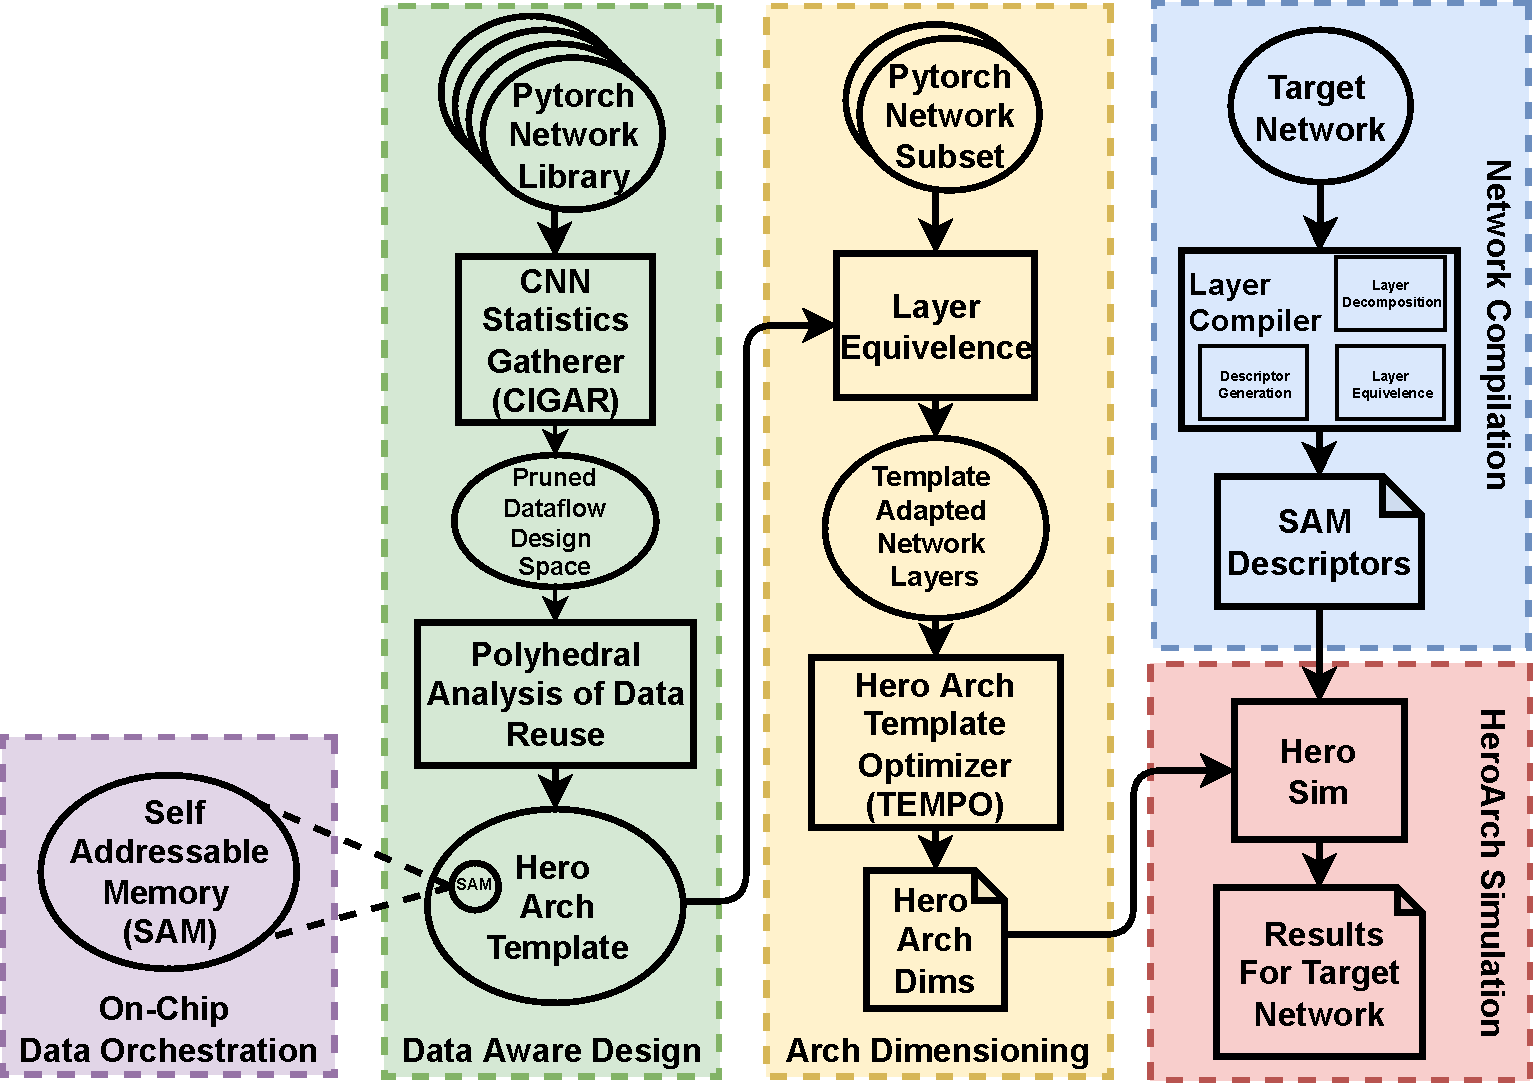
\includegraphics[scale=1]{fig/intro.pdf}
  \caption{Visual illustration of the solution overview}
  \label{fig:intro}
\end{figure}


The full solution overview is presented in \autoref{fig:intro}. This thesis
presents (HERO), a Hybrid GEMM and Direct Convolution Accelerator.  
HERO supports general matrix multiplication to maintain generality across
different network layers. General matrix multiplication is the backbone of many
computationally intensive layers in modern DNNs, for example, self attention
layers in transformer networks \cite{transformer_model} as well as fully
connected layers in many CNNs like Resnet \cite{resnet}. Extending support to
GEMM should not detract from the primary goal of accelerating convolutions since
they represent a larger portion of most network's runtime.  
HERO is derived from a data aware design process. It is optimized for the common
case of convolutions in the literature by supporting these convolution
configurations directly without the need to convert them into GEMM using data
transformation techniques like Im2Col.


HERO's design is data-aware, optimized for the common case of convolutions by
supporting common configurations directly without the need for conversion
techniques like Im2Col. To identify the common case of convolutions, this thesis
introduces CIGAR, a tool that can gather configuration statistics for
convolution and linear layers in a library of DNNs written in \cite{pytorch}. CIGAR can
analyze a network or a library of networks and reveal the most common
convolution layer configurations across the entire library. The networks
analyzed by CIGAR are provided by the \cite{timm} python library of networks, which has
over 695 networks written in PyTorch available for analysis. Any layer configurations
not supported directly by HERO are converted into equivalent GEMM operations
using data transformation techniques like Im2Col
\cite{cafe_con_troll}.


HERO is more than just a single architecture; it represents a configurable
template with flexible allocation of on-chip compute resources called processing
engines (PEs) used in processing convolution layer channels and filters. This
configurability allows for compile-time optimization of HERO by changing the
number of PEs allocated to processing different channels and filters in a
convolution layer. To determine the optimal configuration, this thesis
introduces TEMPO, a tool that uses analytical models for estimating different
architecture metrics like latency, utilization, and memory access counts when
running different DNNs. TEMPO takes advantage of CIGAR's model dimension
collection to extract configurations of convolution layers and applies the
aforementioned analytical models to them. TEMPO provides the initial
architecture dimensions for the HERO template in order to get the first
estimates for other performance metrics. TEMPO only defines layer dimensions for
channel and filter concurrency. A separate analysis of memory usage for
different convolution elements is provided in this thesis. The networks  used by
TEMPO is the entire TIMM library to find the most general architecture
dimensions for HERO.


Additionally, to manage data movement within the Hybrid GEMM and Direct
Convolution Accelerator (HERO). This thesis introduces the Self-Addressable
Memory (SAM), an on-chip programmable memory primitive. SAMs are programmed
using descriptors that define time-dependent address streams, which, in
combination with sufficiently flexible on-chip communication, provide the
necessary flexibility to map arbitrary network layers onto HERO. SAMs enable for
more efficient data movement on-chip, with the aim of maximizing data reuse. To
determine the reuse behavior in the convolution operation, this thesis applies
the polyhedral model to different data elements in convolution layers, using
techniques outlined in \cite{meeus}. Additionally, this thesis introduces a HERO
network compiler called EMPIRE that aids in the mapping of arbitrary PyTorch
models to SAM descriptors, which drive on-chip data movement.


To evaluate the performance and energy efficiency of HERO, a cycle accurate
simulation platform is developed. This simulation platform is driven by a
SystemC simulation backend and a Python evaluation frontend. The simulation
platform allows for the evaluation of different configurations of HERO on a wide
variety of networks. An analysis of an optimal HERO configuration when running
695 networks from the TIMM library was performed. The HERO configuration
analyzed was found to perform well on a wide variety of network configurations,
achieving a median FPS of ~91 FPS with a median speedup of 4.87X over CPU
baseline. The estimated bandwidth required for the configuration of HERO studied
was 19.65GiB/s which is within the PC4-21300 DDR4 specification. With that
configuration of DRAM, the median inferences/J is 57. The total on-chip area is
estimated at 0.34 $mm^2$.


Overall, HERO provides a high-performance, energy-efficient solution for
accelerating convolution layers in a wide range of DNNs. Its general
architecture and support for GEMM, in addition to its direct support for the
common case of convolution layers, make it a versatile accelerator that can
adapt to changing trends in DNNs. The introduction of CIGAR and the HERO layer
compiler, in addition to the use of SAM, further improves the design process and
ease of use of HERO. The cycle accurate simulation platform developed allows for
the accurate evaluation of HERO's performance


\section{Thesis Structure}
\label{chap:intro:thesis_structure}


In this thesis, Chapter \ref{chap:background:intro} discusses background and
related work in the literature. Chapter \ref{chap:dda} introduces the CIGAR and
the data-aware design approach from which HERO is derived. Chapter
\ref{chap:arch_dimensioning} introduces TEMPO, from which several candidate
configurations of HERO are presented. Chapter \ref{chap:data_orchestration}
introduces the SAM primitive. Chapter \ref{chap:net_compile} discusses HERO's
network compilation process and how SAM descriptors are generated from arbitrary
models in Pytorch using EMPIRE. Finally, Chapter \ref{chap:hero:sim_platform}
discusses the HERO simulation platform as well as results from running a HERO
configuration optimized by TEMPO on all 695 networks in the TIMM library.